\documentclass{article}

\usepackage{amsmath, graphics}

\title{Revis\~ao R\'apida de Efeito Fotoel\'etrico}
\author{Rafael Lopes de S\'a}
\date{\today}

\begin{document}
\maketitle

\section{Resumo}

O efeito fotoel\'etrico consiste num el\'etron de um metal absorvendo um f\'oton de forma que esse el\'etron se torna livre:

\begin{equation}
\text{el\'etron ligado} + \text{f\'oton} \rightarrow \text{el\'etron livre}
\end{equation}



Se a energia do f\'oton absorvida pelo el\'etron for maior que a energia de liga\c c\~ao do el\'etron com a estrutura met\'alica, o el\'etron vai se tornar livre e pode formar uma corrente el\'etrica. Quase todo problema sobre efeito fotoel\'etrico se resolve usando conserva\c c\~ao de energia. Conceitualmente:

\begin{equation}
\begin{split}
(\text{energia do f\'oton}) &- (\text{energia gasta para liberar o f\'oton da estrutura met\'alica}) = \\
&(\text{energia cin\'etica do el\'etron livre}) + (\text{energia potencial do el\'etron livre})
\end{split}
\end{equation}

A energia gasta para liberar o f\'oton da estrutura met\'alica \'e algo complicado de se calcular e, em geral, representamos apenas por um s\'imbolo $\phi$ e pelo nome ``fun\c c\~ao trabalho''. \'E uma propriedade do metal e n\~ao do f\'oton.

A energia de um f\'oton \'e proporcional \`a sua freq\"u\^encia:
\begin{equation}
E_f = hf,
\end{equation}
onde $h$ \'e chamado de \textbf{constante de Planck}. A energia cin\'etica \'e dada pela f\'ormula familiar:
\begin{equation}
E_c = \frac{1}{2}mv^2.
\end{equation}
J\'a a energia potencial depende do seu sistema. Usualmente uma bateria pode ser conectada \`a celula fotoel\'etrica criando uma diferen\c ca de potencial. O el\'etron tem que ent\~ao ir de contra (se o polo positivo da bateria estiver ligado ao cotodo) ou a favor (de o polo negativo da bateria estiver ligado ao catodo) esse potencial e gastar\'a ou, respectivamente, receber\'a uma energia dada por:
\begin{equation}
E_p = Q_e\times V,
\end{equation}
onde $Q_e$ \'e a carga do el\'etron e V \'e a diferen\c ca de potencial da bateria. Colocando todos os conceitos juntos:
\begin{equation}\label{eq:energia}
hf - \phi = E_c + E_p = \frac{1}{2}mv^2 + Q_eV.
\end{equation}

Algumas coisas a se lembrar:
\begin{itemize}
\item No efeito fotoel\'etrico usual, cada f\'oton \'e absrovido por um el\'etron. Isso quer dizer que se a energia do f\'oton n\~ao for pelo menos a fun\c c\~ao trabalho $\phi$, n\~ao haver\'a corrente el\'etrica. No caso em que h\'a uma bateria tamb\'em, a energia do f\'oton tem que ser, pelo menos, a fun\c c\~ao trabalho mais a energia potencial provida pela bateria.
\item Se o el\'etron absorver um f\'oton de energia maior (isto \'e, de maior frequ\^encia), ele sair\'a com maior energia. Mas \textbf{n\~ao quer dizer que mais el\'etrons ser\~ao emitidos}.
\item Para emitir mais el\'etron, voc\^e precisa de mais f\'otons. Isso quer dizer uma luz incidente mais intensa.
\end{itemize}

\section{Constantes e unidades}

A unidade de energia no Sistema Internacional de unidades \'e o Joule. $1\,\text{J}$ \'e uma quantidade muito grande para efeitos at\^omicos e subat\^omicos. Uma unidade conveniente \'e o $\text{eV}$. 1 $\text{eV}$ \'e definido como a energia que 1 (um) el\'etron tem num potencial de 1 (um) Volt. Para converter para o SI, basta usar a carga do el\'etron:

\begin{itemize}
\item $1\,\text{eV} = 1.6\times 10^{-19}\text{J}$,
\item $1\,\text{J} = 1/(1.6\times 10^{-19})\,\text{eV} = 6.24\times 10^{18}\,\text{eV}$ ,
\end{itemize}
pela pr\'opria defini\c c\~ao de $\text{eV}$ a carga el\'etrica fundamental \'e escrita como $e = 1.6\times 10^{-19}\,\text{C} = 1\,\text{eV/V}$.

Algumas constantes:

\begin{itemize}
\item $h = 6.626\times 10^{-34}\,\text{J s} = 4.136\times 10^{-15}\,\text{eV s}$,
\item $c = 3\times 10^{8}\,\text{m/s}$.
\item $hc = 1240\,\text{eV nm}$
\end{itemize}
O valor de $hc$ \'e conveniente porque, muitas vezes, \'e dado o comprimento de onda ($\lambda$) do f\'oton em vez da freq\"u\^encia. Essas duas quantidades se relacionam por:

\begin{equation}
c = \lambda f,
\end{equation}
logo, a energia de um f\'oton com comprimento de onda $\lambda$ \'e dada por:
\begin{equation}
E = hf = \frac{hc}{\lambda}.
\end{equation}

Algumas vezes tamb\'em \'e conveniente usar $\text{eV/c}^2$ como unidade de massa e $eV/c$ como unidade de momento linear. Nessa unidade, a massa do el\'etron é dada por:
\begin{equation}
m_e = 511\, \text{keV/c}^2.
\end{equation}

\section{Um exemplo t\'ipico}

A figura abaixo representa o arranjo t\'ipico do efeito fotoel\'etrico:

\begin{figure}[h]
\centering
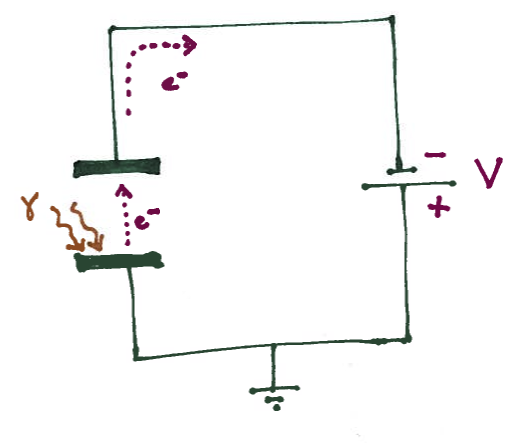
\includegraphics{circuito.png}
\caption{Arranjo t\'ipio do efeito fotoel\'etrico. Note que a luz indice sobre a placa superior, chamada \textbf{anodo}, enquanto a placa inferior, chamada \textbf{catodo}, coleta el\'etrons que percorrerem o circuito completo. Para mais detalhes veja texto.
\end{figure}
A luz incide sobre a placa superior. Se os f\'otons tiverem mais energia que a \textbf{fun\c c\~ao trabalho}, isto \'e, que a energia necess\'aria para liberar os el\'etrons da estrutura met\'alica, esse el\'etrons podem se propagar pelo fio, como representado pela seta pontilhada. Contudo, note que há tamb\'em uma bateria no circuito. Essa bateria faz com que o fio na parte de cima esteja num potencial diferente do fio embaixo. Se assumirmos que o potencial do fio embaixo \'e 0, o potencial do fio de cima ser\'a negativo. Voc\^e pode dizer isso pela orienta\c c\~ao da baterial: veja que o terminal negativo (linha curta) est\'a ligada ao fio de cima.

Como el\'etrons s\~ao negativos e o potencial \'e negativo, os el\'etrons experimental uma for\c ca contra seu movimento. Dito de outra forma, como tanta a carga do el\'etron quando o potencial el\'etrico \'e negativo, ent\~ao a energia potencial do fio em cima:

\begin{equation}
E_p = Q_E\times V > 0,
\end{equation}
\'e positiva. Num an\'alogo gravitacional, \'e como se houvesse uma montanha que os el\'etrons tem que subir. Isto quer dizer que os el\'etrons tem que gastar essa energia para conseguir se propagar no fio. Isso, claro, al\'em da energia gasta para se liberar da estrutura met\'alica (fun\c c\~ao trabalho). Desta forma, a energia cin\'etica do el\'etron \'e dada pela equ\c c\~ao \eqref{eq:energia}:
\begin{equation}
E_c = hf - \phi - Q_e\times V.
\end{equation}
A energia cin\'ética \'e um n\'umero maior ou igual a zero. Quando a energia cin\'etica dos el\'etrons \'e zero, isso quer dizer que n\~ao h\'a corrente el\'etrica. O potencial para o qual isso acontece \'e dado por:
\begin{equation}
0 = hf - \phi - Q_e\times V_{\text{max}}.
\end{equation}
Essa \'e uma maneira muito conveniente de se medir a fun\c c\~ao trabalho de um potencial. Dado que voc\^e sabe a freq\"u\^encia do f\'oton e o potencial da baterial em que a corrente cessa ($V_{\text{max}}$), a fun\c c\~ao taabalho pode ser encontrada resolvendo a equa\c c\~ao acima:
\begin{equation}
\phi = hf - Q_e\times V_{\text{max}}.
\end{equation}


\end{document}
